\subsection{State of System}\label{stateofsystem}

In this section the report discusses the current state of the system in the fulfillment of the curriculum's and personally imposed requirements, both functional and non-functional. 


\subsubsection*{Non-functional}
The non-functional requirements are derived from the curriculum, generic requirement description combined with personal choices of software and measures. They are enlisted as follows:

\begin{enumerate}[noitemsep]
  \item Maintainability through scanning project using Sonarcloud.
  \item 2 static analysis NuGet packages "AsyncFixer", "SonarAnalyzer".
  \item Scanning docker containers for vulnerabilities.
  \item The project must pass all test cases.
\end{enumerate}

Sonarcloud — a maintenance tool detecting technical debt and known security vulnerabilities — has continuously helped the team find security vulnerabilities and insufficient code. If the project was to further developed, there were still code smells remaining to fix to lower any technical debt.

\begin{figure}[h]
    \centering
    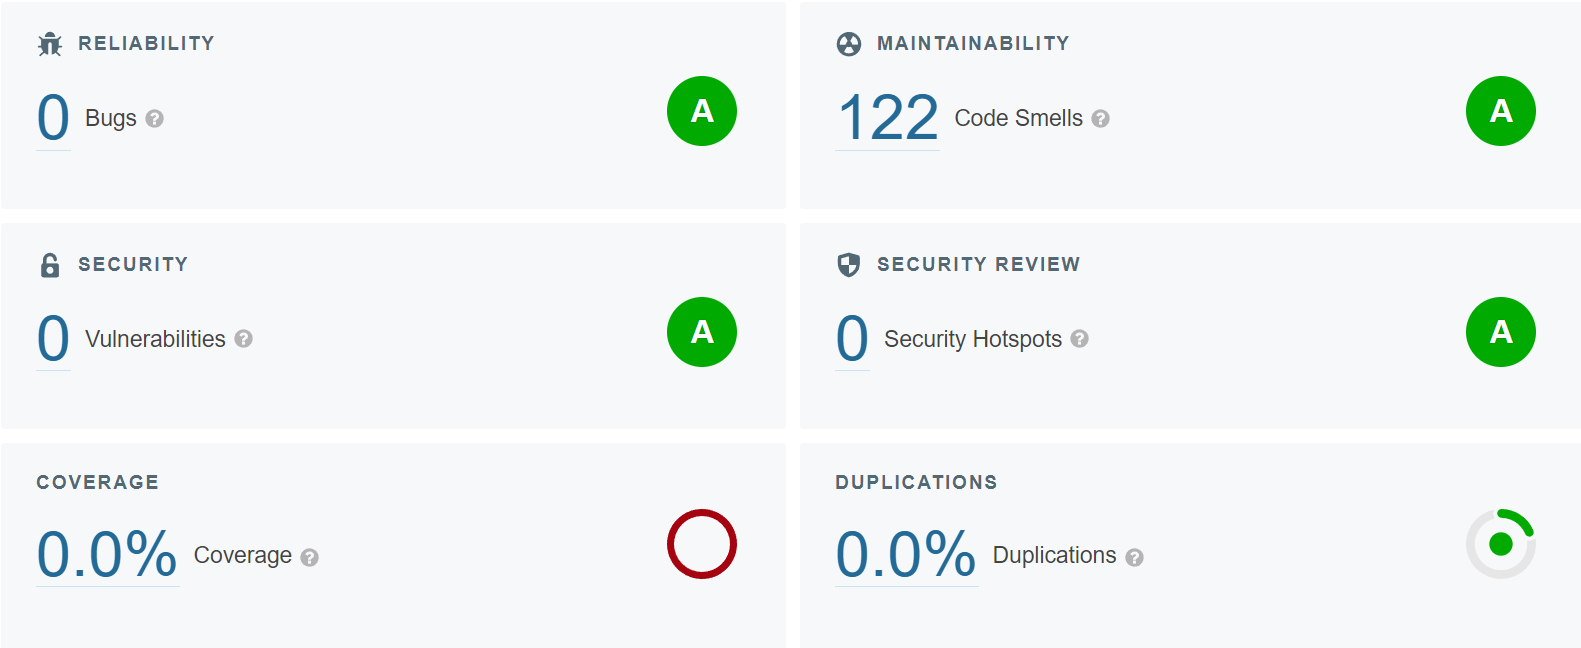
\includegraphics[width=0.8\textwidth]{images/sonarscan.PNG}
    \caption{SonarCloud scan dashboard.}
    \label{fig:scanCode}
\end{figure}

The current ratings has reassured the team that the practices agreed upon are held up and implemented rather correctly. The team aimed to structure the codebase using SE practices such as interface programming code, low cyclomatic complexity, single responsibility, low couplings, and high cohesion. It was essential to write structured code in case changes occurred. As for static analysis, the project would fail its build, if the analyzers found any flaws. The "AsyncFixer" package finds flaws in async calls, which would be a good addition to this REST-API project. The "SonarAnalyzer" spots apparent bugs and known security vulnerabilities. The project can not build if either of the analyzers detect any issues. 

\vspace{3mm}

In addition to the analyzers, the docker containers get scanned using "docker scan" prior to any deployments and stops any build containing a "critical vulnerability". The team wrote a regex script that analyzed the docker scan's output to accomplish this feature~\cite{dockerScanner}. Lastly, the project must also pass all unit tests. The project currently contains 27 test cases, but the test suite should be improved and be more thorough, if the project is to become a real-world application. The team felt the importance of test cases to ensure no functionality breaks when implementing new features or trying to optimize the code.

\subsubsection*{Functional}

The functional requirements can be described as it is the ability to support the functionality of the frontend, together with minimized error-responses from simulator requests.
\vspace{3mm}

\underline{Frontend}

All required functional requirements are implemented in the frontend: users can follow, twit, delete twits, and observe the main page. However, a contract between the frontend and backend could have been beneficial. It occurred that changes had to be made multiple times to get everything working flawlessly. A contract is a powerful tool to settle expectations from both front- and backend, which makes it easy to implement adjustments according to precise specification of requirements with no confusion.
\vspace{3mm}

\underline{Simulator}

The simulator was returning errors for a few weeks. Initially, the implemented functionality was incorrect. Progress occurred as the team implemented a simple logging system on our Digital Ocean server, which enabled the team  to analyze the errors/status codes. Once the status codes were correctly implemented, a new problem arose; the database did not contain all the simulator's users due to the backend mishandling initial user registrations. The lack of users resulted in continuous errors as the simulator expected them to be present. To stop the errors, a SQL dump was requested from another group, followed by a creation of a script that translated the data into JSON objects. This data was then sent to our API one at a time through post requests. Upon completion, the simulator stopped detecting errors. Towards the end, the simulator began detecting "Read timeouts", which we overcame by scaling the project using Docker Swarm. Eventually, the simulator requirements were fulfilled.